\section{Induced Topologies} 

\subsection{Initial and Final Topologies} 

  We have seen some examples of how to create topologies. They can be created without any assumptions on the set, such as the discrete, indiscrete, and the cofinite topologies. More often, we want to consider how a certain structure like the order or a metric induces a topology. Now, we will consider how \textit{functions} can induce a topology. The uniqueness of such induced topologies is called the \textit{universal property}. 

  \begin{definition}[Initial Topology]
    Given a space $X$ and a family of topological spaces $\{Y_\alpha\}_{\alpha \in A}$ 
    \begin{equation}
      f_i : X \rightarrow (Y_\alpha, \T_\alpha)
    \end{equation} 
    the \textbf{initial topology} on $X$ is the coarsest topology $\T$ on $X$ s.t. that each 
    \begin{equation}
      f_i (X, \T) \rightarrow (Y_\alpha, \T_\alpha)
    \end{equation}
    is continuous. 
  \end{definition}

  \begin{definition}[Final Topology]
    Given a space $Y$ and a family of topological spaces $\{X_\alpha\}_{\alpha \in A}$ 
    \begin{equation}
      f: (X, \T_\alpha) \rightarrow Y
    \end{equation}
    the \textbf{final topology} on $Y$ is the finest topology $\T$ on $Y$ s.t. each 
    \begin{equation}
      f: (X, \T_\alpha) \rightarrow (Y, \T)
    \end{equation}
    is continuous. 
  \end{definition}

  Note that it makes sense to talk about the coarsest topology on the domain and the finest topology on the codomain. If it were the other way around, i.e. the finest topology on the domain, then the initial topology on $X$ would be the discrete topology, making every function defined on $X$ continuous. In the same logic, the coarsest topology on $Y$ would trivially be the trivial topology, making all $Y$-valued functions continuous. With these current definitions, if $\T_Y$ is too fine (e.g. if $\T_Y = 2^Y$), then the open sets of $\T_Y$ would be too fine and therefore would have a preimage that may not be open in $X$. 

\subsection{Subspace Topology} 

  The reason we want to do this is because we want to think of $Y$ as its own entity, independent of $X$. 

  \begin{definition}[Subspace Topology]
    Given topological space $X$ and subspace $Y \subset X$, the \textbf{subspace topology} on $Y$ is defined in the equivalent ways. 
    \begin{enumerate}
      \item It is the initial topology on the subspace with respect to the inclusion map $\iota: Y \rightarrow X$. 
      \item It is the topology consisting of $X$-open sets intersection $Y$. 
      \begin{equation}
        \T_Y = \{(U \cap Y) \subset Y \mid U \in \T_X\}
      \end{equation}
    \end{enumerate}

    \begin{figure}[H]
      \centering 
      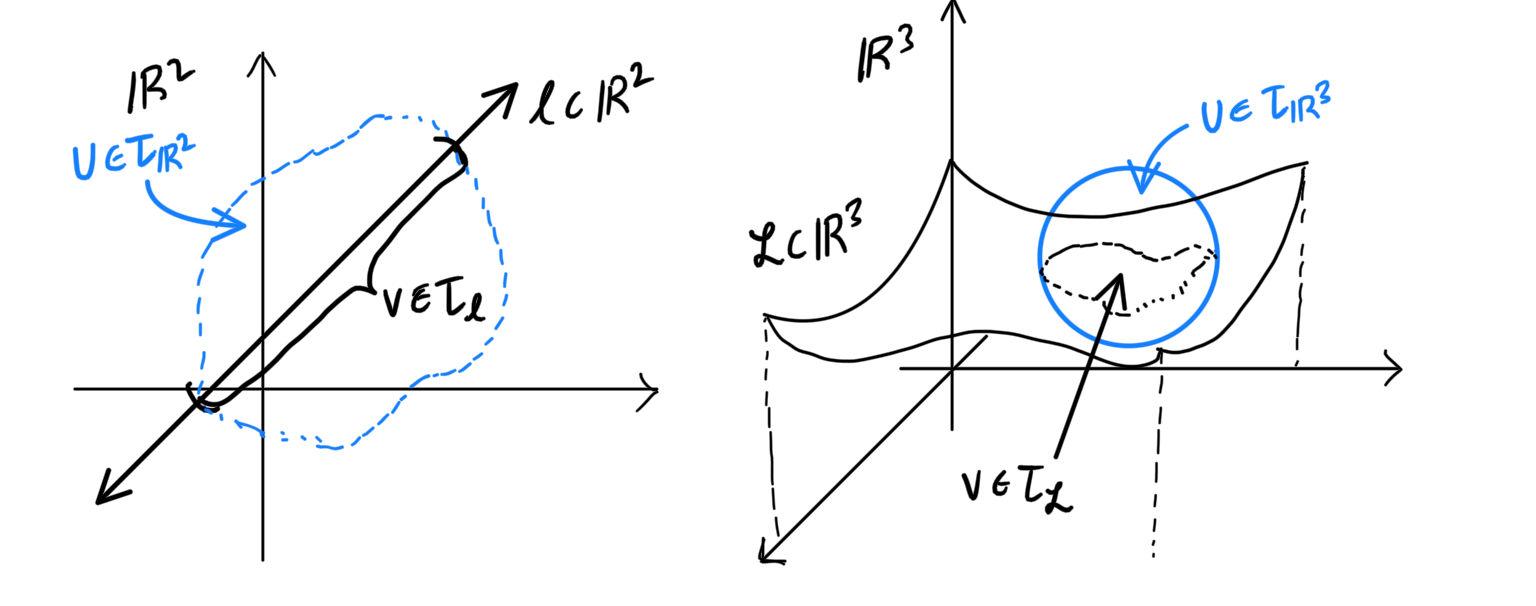
\includegraphics[scale=0.4]{img/Subspace_Topology.png}
      \caption{The subspace topology of a line $l$ embedded in $\mathbb{R}^2$ and that of a surface $\mathcal{L}$ embedded in $\mathbb{R}^3$ is shown.}
      \label{fig:subspace_topology}
    \end{figure} 
  \end{definition} 
  \begin{proof}
    We prove the properties. 
    \begin{enumerate}
      \item \textit{Trivial}. We see that $\emptyset = \emptyset \cap Y$ and $Y = X \cap Y$. 
      \item \textit{Stability under Union}. Suppose $\{V_\alpha\}_{\alpha \in A}$ are setes that are open in $Y$. Then for each $\alpha$ there exists an open set $U_\alpha \subset X$ that is open in $X$. Therefore, 
      \begin{align}
        \bigcup_{\alpha \in A} V_\alpha & = \bigcup_{\alpha \in A} (U_\alpha \cap Y) \\ 
                                        & = Y \cap \bigg( \bigcup_{\alpha \in A} U_\alpha \bigg)
      \end{align}
      where $\cup_\alpha U_\alpha$ is open in $X$, and therefore we shown that there exists such an open set. 

      \item \textit{Stability under Finite Intersection}. Suppose $\{V_i\}_{i = 1}^n$ are open in $Y$. Then we can do the same thing. 
    \end{enumerate}
  \end{proof}

  Consider any set $U \subset Y$. Note that if $U$ is an open set in $X$ that happens to be contained in $Y$, then we can set $U = U \cap Y$, so $U$ is open in $Y$. However, we have seen that being open in $Y$ does not necessarily imply that it is open in $X$. 

  \begin{example}[Non-Open Sets may be Open in Subspace]
    Let $X = \mathbb{R}$ with the Euclidean topology and let $Y = [0, 1]$. 
    \begin{enumerate}
      \item $[0, 1]$ is open in $Y$ but not in $X$. 
      \item Intervals of the form $(a, 1]$ and $[0, b)$ are open in $Y$ but not in $X$. 
    \end{enumerate}
  \end{example} 

  \begin{example}[Singleton Sets in Subspace Topologies]
    Consider $X = \mathbb{R}$ with the lower limit topology with $Y = [0, 1]$. The following 
    \begin{enumerate}
      \item $[1/2, 1] = Y \cap [1/2, 2)$, and 
      \item $\{1\} = Y \cap [1, 2)$
    \end{enumerate}
    are open in the subspace topology. It turns out that $\{1\}$ is the only singleton set open in $Y$. 
  \end{example}

  Furthermore, we can immediately retrieve the basis of the subspace topology. 

  \begin{theorem}[Induced Basis of Subspace Topologies]
    If $\B$ is a basis for the topology of $X$, then 
    \begin{equation}
      \B_Y \coloneqq \{B \cap Y \mid B \in \B \} 
    \end{equation}
    is a basis for the subspace topology of $Y$. 
  \end{theorem}
  \begin{proof}
    
  \end{proof}

  Let's go through a few examples. 

  \begin{example}[Closed Unit Interval in $\mathbb{R}$]
    The basis for the subspace topology of $[0, 1] \subset \mathbb{R}$ with the Euclidean topology consists of the intervals 
    \begin{enumerate}
      \item $(a, b)$ where $0 \leq a < b \leq 1$. 
      \item $[0, b)$ where $0 < b \leq 1$. 
      \item $(a, 1]$ where $0 \leq a < 1$. 
    \end{enumerate}
  \end{example} 

  \begin{example}[Unit Sphere in $\mathbb{R}^n$] 
    Let $S^n \subset \mathbb{R}^{n+1}$ be the unit \textbf{n-sphere} defined $S^n \coloneqq \{x \in \mathbb{R}^{n+1} \mid ||x||^2 = 1 \}$. When thinking about $S^n$ as a space itself, we use the subspace topology coming from the standard topology of $\mathbb{R}^n$. 
  \end{example}

  \begin{example}[$S^1 \subset \mathbb{R}^2$]
    Let's focus on $n = 1$. For $a < b$, let 
    \begin{equation}
      A_{a, b} = \{ (\cos{t}, \sin{t}) \mid a < t < b \}
    \end{equation} 
    Then, we can see that
    \begin{enumerate}
      \item if $b - a > 2 \pi$, then $A_{a, b} = S^1$. 
      \item If $b - a \leq 2 \pi$, then $A_{a, b}$ is an ``open arc'' from $(\cos{a}, \sin{a})$ to $(\cos{b}, \sin{b})$.  
    \end{enumerate} 

    Given that we have an equivalence class defined 
    \begin{equation}
      A_{a, b} \sim A_{a + 2 \pi k, b + 2 \pi k} \text{ for all } k \in \mathbb{Z}
    \end{equation} 
    We claim that $\{A_{a, b}\}$ is a basis for the subspace topology of $S^1$. We can see that the open arc covering the top right quadrant in $\mathbb{R}^2$ is 
    \begin{equation}
      S^1 \cap (0, 1)^2 = S^1 \cap B_\infty \big( (\frac{1}{2}, \frac{1}{2}), \frac{1}{2} \big)
    \end{equation}
  \end{example}

  Now let's focus more on metric spaces. Note that if we want to construct topologies of subspaces of metric spaces, there are two ways to do it. It would be quite bad if these resulted in different topologies, but fortunately we have the following theorem. 

  \begin{theorem}[Topologies on Subspaces of Metric Spaces Coincide]
    Let $(X, d_X)$ be a metric space, with $Y \subset X$. There are 2 ways we can define a topology on $Y$. 
    \begin{enumerate}
      \item Take the metric topology $\T_X$ on $X$, and then take the subspace topology on $Y$. 
      \item Induce a metric $d_Y = d_{X | Y}$ on $Y$ which is a restriction of $d_X$ to $Y$, and then take the metric topology of it. 
    \end{enumerate}
    We claim that these two constructions give the same topology, as shown in the commutative diagram. 

    \begin{figure}[H]
      \centering 
      \begin{tikzcd}
        d_X \arrow[r] \arrow[d] & d_Y \arrow[d] \\
        \T_X \arrow[r] & \T_Y 
      \end{tikzcd}
      \caption{} 
      \label{fig:same_construction}
    \end{figure}
  \end{theorem}
  \begin{proof}
    The basis for the subspace topology on $Y$ is 
    \begin{equation}
      \B_1 = \{B_{d_X} (x, r) \cap Y \mid x \in X, r > 0 \}
    \end{equation} 
    and the basis for the (induced) metric topology on $Y$ is 
    \begin{equation}
      \B_2 = \{B_{d_Y} (y, r) \cap Y \mid y \in Y, r > 0 \} = \{B_{d_X} (y, r) \cap Y \mid y \in Y, r > 0 \}
    \end{equation} 
    It is immediate that $\B_2 \subset \B_1$ since it goes over all $x \in X$ rather than $y \in Y$. To see why $\B_1 \subset \B_2$, TBD. 
  \end{proof}

  \begin{theorem}[Closures in Subspace Topologies]
    Let $A \subset Y \subset X$. Let $\bar{A}$ denote the closure of $A$ in $X$. Then, the closure of $A$ in $Y$ equals $\bar{A} \cap Y$. 
  \end{theorem}

\subsection{Box Topology} 

  There are multiple ways to define the box and product topologies, but their construction with basis elements is most simple. 

  \begin{definition}[Box Topology]
    Given a family of topological spaces $\{(X_\alpha, \T_\alpha)\}_{\alpha \in A}$, the \textbf{box topology} on the space $\prod_{\alpha \in A} X_\alpha$ is the topology generated by the basis 
    \begin{equation}
      \mathscr{B} = \bigg\{ \prod_{\alpha \in A} U_\alpha \mid U_\alpha \in \T_\alpha \bigg\}
    \end{equation}

    \begin{figure}[H]
      \centering 
      \begin{tikzpicture}
        \draw[<->] (-1,0)--(6,0);
        \draw[<->] (0,-1)--(0,4);
        \draw[dashed] (1,1)--(1,3)--(4,3)--(4,1)--(1,1);
        \node[below] at (6,0) {$\mathbb{R}$};
        \node[left] at (0,4) {$\mathbb{R}$};
        \node[below] at (1,-0.3) {$a$};
        \node[below] at (4,-0.3) {$b$};
        \node[left] at (-0.3,1) {$c$};
        \node[left] at (-0.3,3) {$d$};
        \node[rotate=90] at (0,1) {$($};
        \node[rotate=-90] at (0,3) {$($};
        \node at (1,0) {$($};
        \node at (4,0) {$)$};
      \end{tikzpicture}
      \caption{We can visualize the elements of the box topology with the product space $\mathbb{R}^2 = \mathbb{R} \times \mathbb{R}$, where each $\mathbb{R}$ has an open ball topology. From the visual below, we can see why this is called the "box" topology. }
      \label{fig:box_topology}
    \end{figure}
  \end{definition}
  \begin{proof}
    It is easy to prove that the box topology indeed satisfies the 3 properties of topologies in general. 
  \end{proof}

\subsection{Product Topology}

  While the box topology may seem quite "intuitive" for the first learner, the box topology however, has serious limitations when extending to infinite Cartesian products of spaces. The main difference between the construction of open sets in the box topology vs the product topology is that the box topology merely describes open sets as direct products of open sets from each coordinate space while the construction of the product topology is completely dependent on the construction of the projection mappings 
  \begin{equation}
    \pi_\beta: \prod_{\alpha \in I} X_\alpha \rightarrow X_\beta
  \end{equation}
  to be continuous (and nothing more) so that (by definition) the preimages of open sets in $X_\beta$ under $\pi_\beta$ are open sets in $\prod X_\alpha$. Therefore, the construction of the continuous $\pi_\beta$'s canonically constructs a basis of open sets in $\prod X_\alpha$. 

  \begin{definition}[Product Topology] 
    Given a family of topological spaces $\{(X_\alpha, \T_\alpha)\}_{\alpha \in A}$, the \textbf{product topology} on the space $\prod_{\alpha \in A} X_\alpha$ is defined in the following equivalent ways. 
    \begin{enumerate}
      \item It is the initial topology on the product space wrt the family of projections $p_\alpha: \prod_{\alpha \in A} X_\alpha \rightarrow X_\alpha$. 

      \item It is the topology generated by the basis of elements 
      \begin{equation}
        \prod_\alpha U_\alpha 
      \end{equation}
      where $U_\alpha$ is a proper open subset for at most finitely many $\alpha$'s, and $U_\alpha = X_\alpha$ for all other $\alpha$. 
    \end{enumerate}

    \begin{figure}[H]
      \centering 
      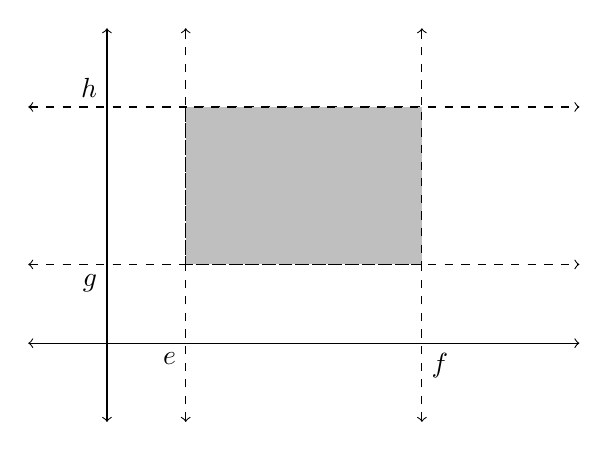
\begin{tikzpicture}
        \draw[<->] (-1,0)--(6,0);
        \draw[<->] (0,-1)--(0,4);
        \draw[<->, dashed] (-1,1)--(6,1);
        \draw[<->, dashed] (-1,3)--(6,3);
        \draw[<->, dashed] (1,-1)--(1,4);
        \draw[<->, dashed] (4,-1)--(4,4);
        \node [below left] at (1,0) {$e$};
        \node [below right] at (4,0) {$f$};
        \node [above left] at (0,3) {$h$};
        \node [below left] at (0,1) {$g$};
        \draw[dashed, fill=lightgray] (1,1) rectangle (4,3);
      \end{tikzpicture}
      \caption{Visually, we can interpret each $\mathscr{S} (U_\beta)$ as a "strip" in the total product space. For example in $\mathbb{R}^2$, there are two "strips" $(e, f) \times \mathbb{R}$ and $\mathbb{R} \times (g, h)$ that intersect. Note that each strip is the preimage of the projection mapping. }
      \label{fig:product_topology}
    \end{figure}
  \end{definition}

  We can deduce some conclusions comparing these topologies. First, the product and box topologies are precisely the same if we work in finite Cartesian products of spaces, since any element of the box topology (left hand side) can be expressed as a finite intersection of some open sets (in the right hand side). That is, if $\text{card}\,I < \infty$, then 
  \begin{equation}
    \prod_{\alpha \in I} U_i = \bigcap_{\alpha \in I} \big\{ \prod_{\gamma \in I} W_\gamma \; | \; W_\gamma = U_\gamma \text{ if } \gamma = \alpha, \, W_\gamma = X_\gamma \text{ if } \gamma \neq \alpha\big\}
  \end{equation}
  Secondly, we can see that the box topology is finer than the product topology (strictly finer if working in infinite product spaces). 

  \begin{example}
    The set $(0,1)^\mathbb{N} \subset \mathbb{R}^\mathbb{N}$ is clearly open in the box topology, but it is considered "too tight" to be in the product topology. However, 
    \begin{equation}
      (0,1) \times \mathbb{R} \times \mathbb{R} \times \ldots
    \end{equation}
    is open in the product topology since only one (a finite amount) of the factors is not the whole space. 
  \end{example}

  The following theorem reveals why the product topology is superior than the box topology in product spaces. 

  \begin{theorem}[Continuity of Functions Mapped to Product Topology]
    Given the function 
    \begin{equation}
      f: A \rightarrow \prod_{\alpha \in I} X_\alpha, \; f(a) \equiv \big( f_\alpha (a) \big)_{\alpha \in I}
    \end{equation}
    with its component functions $f_\alpha: A \rightarrow X_\alpha$. Let $\prod X_\alpha$ have the product topology. Then the function $f$ is continuous if and only if each function $f_\alpha$ is continuous. 
  \end{theorem}
  \begin{proof}
    We prove both directions. Let $\pi_\beta$ be the projection of this product onto the $\beta$th component space. By construction $\pi_\beta$ is continuous $\implies \pi_\beta^{-1} (U_\beta)$ is a basis element of the product topology of $\prod X_\alpha$. 
    \begin{enumerate}
      \item $(\rightarrow)$ $f$ is continuous, so $f_\beta \equiv \pi_\beta \circ f$, as the composition of continuous functions, is also continuous. 
      \item $(\leftarrow)$ Assume that each $f_\beta$ is continuous. Let there be an open set $U_\beta \subset X_\beta$. Then, the canonical open set $\pi_\beta^{-1}$ in the product space $\prod X_\alpha$ is also open. Now, the preimage of $\pi_\beta^{-1} (U_\beta)$ under $f$ is 
      \begin{align*}
        f^{-1} \big( \pi_\beta^{-1} (U_\beta)\big) & = (f^{-1} \circ \pi_\beta^{-1})(U_\beta) \\
        & = (\pi_\beta \circ f)^{-1} (U_\beta) \\
        & = f_\beta^{-1} (U_\beta)
      \end{align*}
      Since $f_\beta$ is already assumed to be continuous, $f_\beta^{-1} (U_\beta)$ is open in $A$. 
    \end{enumerate}
  \end{proof} 

  This theorem also works for the box topology only if we are working with finite product spaces. But in general, this theorem fails for the box topology. Consider the following example. 

  \begin{example}
    Let $\mathbb{R}^\omega$ be the countably infinite product of $\mathbb{R}$'s. Let us define the function 
    \begin{equation}
      f: \mathbb{R} \rightarrow \mathbb{R}^\omega
    \end{equation}
    with coordinate function defined $f_n (t) \equiv t$ for all $n \in \mathbb{N}$. Clearly, each $f_n$ is continuous. Given the box topology, we consider one basis element of $\mathbb{R}^\omega$
    \begin{equation}
      B = \prod_{i=1}^\infty (-\frac{1}{i}, \frac{1}{i})
    \end{equation}
    Assume that $f$ is continuous, that is $f^{-1}(B)$ is open in $\mathbb{R}$. Then, it would contain some finite interval $(-\delta, \delta)$ about $0$, meaning that $f\big( (-\delta, \delta)\big) \subset B$. This implies that for each $n \in \mathbb{N}$, 
    \begin{equation}
      f_n \big( (-\delta, \delta) \big) = (-\delta, \delta) \subset \Big( -\frac{1}{n}, \frac{1}{n} \Big)
    \end{equation}
    which contradicts the fact that $B$ is open, since the interval $(-1/n, 1/n)$ converges onto a point $0$. 
  \end{example}

  However, there is no useful criterion for the continuity of a mapping $f: X \times Y \longrightarrow A$ even if we have the product topology on $X \times Y$. One might conjecture that this $f$ is continuous if it is continuous in each variable separately, but this is in fact not true. 

  \begin{theorem}[Topologies on Products of Metric Spaces Coincide]
    Given a metric space
  \end{theorem}

  \begin{corollary}
    The Euclidean topology on $\mathbb{R}^n$ is equivalent to the product topology of the Euclidean topologies on $\mathbb{R}$. 
  \end{corollary}

  \begin{lemma}
    The addition, subtraction, and multiplication operations are continuous functions from $\mathbb{R} \times \mathbb{R} \longrightarrow \mathbb{R}$, and the quotient operation is a continuous function from $\mathbb{R} \times (\mathbb{R} \setminus \{0\}) \longrightarrow \mathbb{R}$. 
  \end{lemma}
  \begin{proof}
    Standard $\epsilon-\delta$ proof. 
  \end{proof}

  Now that we have defined what it means for binary operations to be continuous, we can talk about \textit{topological algebra}, which is the study of algebraic structures such that their algebraic operations and inverses are continuous. One important such concept is a \textit{topological group}, which will be mentioned later. 

\subsection{Quotient Topologies}

  \begin{definition}[Quotient Map]
    Let $X$ and $Y$ be topological spaces, and let $p: X \rightarrow Y$ be a surjective map. The map $p$ is said to be a \textbf{quotient map} if
    \begin{equation}
      U \text{ is open in } Y \iff p^{-1}(U) \text{ is open in } X
    \end{equation}
  \end{definition}

  Note that the conditions for being a quotient map is stronger then regular continuity. It is sometimes called \textbf{strong continuity}. An equivalent condition for $p$ to be a quotient map is to require that given $A \subset Y$, 
  \begin{equation}
    A \text{ closed in } Y \iff p^{-1}(A) \text{ closed in } X
  \end{equation}
  This equivalence follows from the fact that
  \begin{equation}
    f^{-1}(Y \setminus B) = X \setminus f^{-1}(B)
  \end{equation}

  \begin{definition}[Saturation]
    A subset $C \subset X$ is \textbf{saturated} with respect to the surjective map $p: X \rightarrow Y$ if for every $p^{-1} (A)$ (where $A \subset Y$) that intersects $C$, $p^{-1}(A)$ is completely contained within $C$. That is, 
    \begin{equation}
      p^{-1} \big( p(C) \big) = C
    \end{equation}

    \begin{figure}[H]
      \centering 
      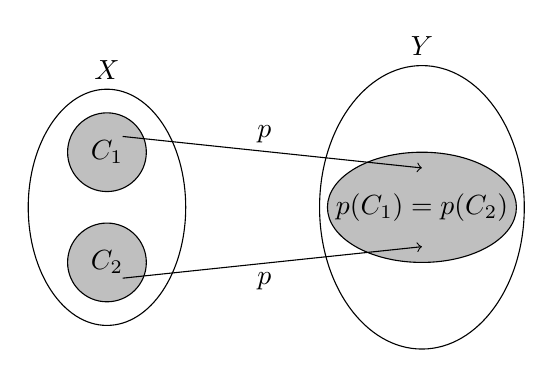
\begin{tikzpicture}
        \draw (0,0) ellipse (1 and 1.5);
        \draw[fill=lightgray] (0, 0.7) circle (0.5);
        \draw[fill=lightgray] (0, -0.7) circle (0.5);
        \node[above] at (0,1.5) {$X$};
        \draw (4,0) ellipse (1.3 and 1.8);
        \node[above] at (4,1.8) {$Y$};
        \draw[fill=lightgray] (4,0) ellipse (1.2 and 0.7);
        \node at (0, 0.7) {$C_1$};
        \node at (0,-0.7) {$C_2$};
        \node at (4,0) {$p(C_1) = p(C_2)$};
        \draw[->] (0.2,0.9)--(4,0.5);
        \draw[->] (0.2,-0.9)--(4,-0.5);
        \node[above] at (2, 0.7) {$p$};
        \node[below] at (2, -0.7) {$p$};
      \end{tikzpicture}
      \caption{We can see that $C_1$ and $C_2$ alone are not saturated, but $C_1 \cup C_2$ is saturated. Visually, for a given set $C \subset X$ to be saturated, there cannot be any points $q \not\in C$ such that $q \in p(C)$. }
      \label{fig:saturation}
    \end{figure}
  \end{definition}

  We now introduce an alternative, equivalent definition of quotient maps. 

  \begin{theorem}
    $p: X \rightarrow Y$ is a quotient map if and only if $p$ is continuous and $p$ maps saturated open sets of $X$ to open sets of $Y$ (or saturated closed sets of $X$ to closed sets of $Y$). 
  \end{theorem}

  \begin{proposition}
    If $p: X \rightarrow Y$ is a surjective, continuous map that is either open or closed (that is, maps open sets to open sets or closed sets to closed sets), then $p$ is a quotient map.\footnote{Note however, that the converse is not true; there exists quotient maps that are neither open nor closed. }
  \end{proposition}

  \begin{definition}
    If $X$ is a space and $A$ is a set and if $p: X \rightarrow A$ is a surjective map, then there exists exactly one topology $\T$ on $A$ relative to which $p$ is a quotient map. $\T$ is called the \textbf{quotient topology} induced by $p$. 
  \end{definition}

  To construct the quotient topology for the surjective map $p$, we must make $p$ continuous. Therfore, the topology $\T$ on $A$ is defined by letting it consist of all subsets $U$ of $A$ such that $p^{-1}(U)$ is open in $X$. This is indeed a topology since
  \begin{enumerate}
    \item $p^{-1} (\emptyset) = \emptyset$ and $p^{-1}(A) = X$
    \item $p^{-1} \Big( \bigcup_{\alpha \in J} U_\alpha \Big) = \bigcup_{\alpha \in J} p^{-1} (U_\alpha)$
    \item $p^{-1} \Big( \bigcap_{i=1}^n U_i \Big) = \bigcap_{i=1}^n p^{-1} (U_i)$
  \end{enumerate}

  \begin{example}
    Let $p: (\mathbb{R}, \T_\mathbb{R}) \rightarrow \mathbb{R} / 2 \pi \mathbb{R}$. Then, the final topology of $\mathbb{R} / 2 \pi \mathbb{R}$ would be simply defined 
    \begin{equation}
      \T_{\mathbb{R} / 2 \pi \mathbb{R}} \equiv \{U \subset \mathbb{R} / 2\pi \mathbb{R} \; | \; U = p(O), O \in \T_\mathbb{R}\}
    \end{equation}
    That is, the quotient topology is merely the set of all images of open sets in $\mathbb{R}$ under $f$. However, if $\mathbb{R} / 2 \pi \mathbb{R}$ has the discrete topology $2^X$, then a single equivalence class, say $[0]$, will get mapped to the collection of points $\{2 \pi k \mid k \in \mathbb{Z}\}$, which is clearly not open in $\mathbb{R}$. Note that the final topology (or the quotient topology) is endowed onto the codomain in order to make $f$ continuous (or a quotient mapping). 
  \end{example}

  \begin{proposition}
    Given a relation $\sim$ on a topological space $(X, \T_X)$, the quotient topology of the quotient space $X / \sim$, is precisely the final topology on the quotient set with respect to the quotient map $p: X \rightarrow X / \sim$. That is, 
    \begin{equation}
      \T_{X / \sim} \equiv \big\{U \subseteq X / \sim \; | \; \{x \in X \; | \; p(x) \in U\} \in \T_X \big\}
    \end{equation}
    which is the topology whose open sets are the subsets of $X / \sim$ that have an open preimage under the surjective map $p: x \mapsto [x]$. 
  \end{proposition}

  \begin{example}
    Let $X \equiv [0,1] \cap [2,3] \subset \mathbb{R}$ and $Y y \equiv [0,2] \subset \mathbb{R}$. Then, we define $p: X \rightarrow Y$ as 
    \begin{equation}
      p(x) \equiv \begin{cases} x & x \in [0,1] \\ x-1 & x \in [2,3] \end{cases}
    \end{equation}
    $p$ is continuous (under subspace topology of $X \subset \mathbb{R}$), surjective, and closed, meaning that it is a quotient map. However, it is not open, since the image of the open set $[0,1]$ of $X$ is $[0,1]$, which is not open in $Y$. 
  \end{example}

  \begin{example}
    Let $p: \mathbb{R} \rightarrow \{a, b, c\}$ be defined as 
    \begin{equation}
      p(x) \equiv \begin{cases} a & x > 0 \\ b & x < 0 \\ c & x = 0 \end{cases}
    \end{equation}
    Then, the quotient topology of $\{a, b, c\}$ consists of 
    \begin{equation}
      \emptyset, \{a\}, \{b\}, \{a, b\}, \{a, b, c\}
    \end{equation}
  \end{example}

  \begin{definition}[Quotient Space]
    Let $X$ be a topological space, and let $\Tilde{X}$ be a partition of $X$ into disjoint subsets whose union is $X$. Let $p: X \rightarrow \Tilde{X}$ be the surjective map mapping every point $x \in X$ to the subset that it is in. In the quotient topology induced by $p$, $\Tilde{X}$ is called the \textbf{quotient space} of $X$. 
  \end{definition}

  To construct a quotient space, we can equivalently define a relation on $X$. That is, a subset $U$ of $\Tilde{X}$ is a collection of equivalence classes, and the set $p^{-1}(U)$ is the union of equivalence classes belonging to $U$. Therefore, the typical open set of $\Tilde{X}$ is a collection of equivalence classes whose union is an open set in $X$. 

  \begin{example}[Construction of a Torus]
    Let $X \equiv [0,1] \times [0,1] \subset \mathbb{R}^2$. We define an equivalence relation $Y$ consisting of the equivalence classes
    \begin{align*}
        &\big\{\{(x, y)\} \; | \; 0<x, y<1\big\} \cup \big\{ \{(x, 0), (x,1)\} \; | \; 0<x<1 \big\} \cup \\
        &\big\{ \{(0,y), (1,y)\} \; | \; 0<y<1 \big\} \cup \big\{ \{(0,0), (0,1), (1,0), (1,1)\} \big\}
    \end{align*} 

    \begin{figure}[H]
      \centering 
      \begin{tikzpicture}
        \draw (0,0) rectangle (2,2);
        \draw (3,0) rectangle (5,2);
        \draw (6,0) rectangle (8,2);
        \draw (9,0) rectangle (11,2);
        \draw[dashed] (1, 1.5) circle [radius=0.4];
        \draw[fill] (1, 1.5) circle [radius=0.03];
        \draw[dashed] (3.9,0) arc (0:180: 0.4);
        \draw[dashed] (3.9,2) arc (0:-180:0.4);
        \draw[dashed] (6,1.1) arc (-90:90:0.4);
        \draw[dashed] (8,1.9) arc (90:270:0.4);
        \draw[fill] (3.5,0) circle [radius=0.03];
        \draw[fill] (3.5,2) circle [radius=0.03];
        \draw[fill] (6,1.5) circle [radius=0.03];
        \draw[fill] (8,1.5) circle [radius=0.03];
        \draw[fill] (9,0) circle [radius=0.03];
        \draw[fill] (11,0) circle [radius=0.03];
        \draw[fill] (9,2) circle [radius=0.03];
        \draw[fill] (11,2) circle [radius=0.03];
        \draw[dashed] (9.4,0) arc (0:90:0.4);
        \draw[dashed] (9.4,2) arc (0:-90:0.4);
        \draw[dashed] (11,0.4) arc (90:180:0.4);
        \draw[dashed] (10.6,2) arc (180:270:0.4);
      \end{tikzpicture}
      \caption{The quotient topology of this quotient space consists of open sets of form. } 
      \label{fig:torus_basis}
    \end{figure}
    This quotient space $X / Y$ is homeomorphic to the torus $S^1 \times S^1$, denoted
    \begin{equation}
      \frac{X}{Y} \cong S^1 \times S^1
    \end{equation}
    We can visualize the construction of the equivalence relation $Y$ as a "gluing" of the rectangle $X$ by its edges and corners. 

    We can check that this mapping is indeed a quotient map. First, it is clearly surjective. By realizing that individual points on the edge of $[0,1]^2$ are open sets themselves (by the subspace topology), we can prove that this map is indeed open and continuous. 
  \end{example}

  \begin{example}[Construction of the 2-Sphere]
    Let $X$ be the closed unit ball 
    \begin{equation}
      X \equiv \{(x, y) \in \mathbb{R}^2 \; | \; x^2 + y^2 \leq 1\}
    \end{equation}
    and define the equialence classes $R$ as 
    \begin{equation}
      R \equiv \big\{ \{(x, y)\} \; | \; x^2 + y^2 <1 \big\} \cup \{S^1\}
    \end{equation}
    which will consist of open sets of one of the two forms
    \begin{center}
    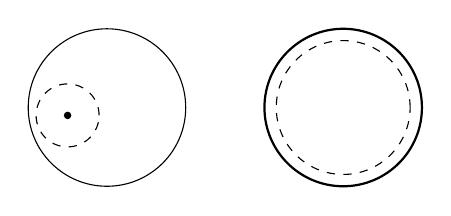
\begin{tikzpicture}
      \draw (1,1) circle [radius=1];
      \draw[thick] (4,1) circle [radius=1];
      \draw[dashed] (0.5,0.9) circle [radius=0.4];
      \draw[fill] (0.5,0.9) circle [radius=0.04];
      \draw[dashed] (4,1) circle [radius=0.85];
    \end{tikzpicture}
    \end{center}
    Then, this quotient space $X / R$ is homeomorphic to the 2-sphere
    \begin{equation}
      S^2 \equiv \{(x, y, z) \in \mathbb{R}^3 \; | \; x^2 + y^2 + z^2 = 1\}
    \end{equation}
    Visually, we can imagine the disk being glued together by its sides to continuously form the 2-sphere. 
  \end{example}

  \begin{example}[Construction of the 1-Sphere]
    We will show that
    \begin{equation}
      \frac{\mathbb{R}}{\mathbb{Z}} \cong S^1
    \end{equation}
    Let us construct the set $(\mathbb{R}, \T_{\mathbb{R}})$ with paramater $t$. We define maps
    \begin{align*}
      p: \mathbb{R} \rightarrow \mathbb{R} / \mathbb{Z}, \;\; p(t) \equiv t \; (\text{mod } 1) \\
      q: \mathbb[R] \rightarrow S^1 \subset \mathbb{C}, \;\; g(t) \equiv e^{2 \pi i t} 
    \end{align*}
    We claim that $p$ and $q$ are both quotient mappings. Clearly, $p$ is a quotient mapping. As for $q$, it it easy to see that it is surjective (but not injective) and continuous ($\T_{S^1}$ has the basis of open intervals on $S^1$). It is also easy to notice that given an open interval $U \subset S^1$, $q^{-1}(U)$ will be the union of open intervals equally spaced in $\mathbb{R}$. Additionally, given any open interval in $\mathbb{R}$, it maps to an open interval in $S^1$ (note that $S^1$ itself is also open). These three conditions imply that $q$ is a quotient map. We now define maps 
    \begin{align}
      q \circ p^{-1}: & \mathbb{R} / \mathbb{Z} \rightarrow S^1 \\
      p \circ q^{-1}: & S^1 \rightarrow \mathbb{R} / \mathbb{Z}
    \end{align}
    and claim that these maps are homeomorphisms. We can clearly see that the mapping from an open set in $\mathbb{R} / \mathbb{Z}$ to the union of spaced open intervals in $\mathbb{R}$ is an injection, and the mapping from this union of open intervals to the union of open intervals in $S^1$ is a surjection. The composition of these two mappings clearly defines a bijection. Therefore, $q \circ p^{-1}$ is proven to be a bicontinuous bijective mapping between open sets $U \subset \mathbb{R} / \mathbb{Z}$ and $V \subset S^1 \implies$ $q \circ p^{-1}$ is a homeomorphism. 

    This result clearly makes sense since 
    \begin{equation}
      \frac{\mathbb{R}}{\mathbb{Z}} \cong \frac{[0,1]}{\sim}
    \end{equation}
    where the relation $\sim$ maps every point $x \in (0,1)$ to its own equivalence class and the points $0, 1$ to one equivalence class $\{0\}$. Therefore, it is informally said that the quotient space of the real line is a circle. 

    One may attempt to construct a simpler set by replacing $S^1$ with the half-open interval $[0,1)$. However, while $[0,1)$ is bijective to $\mathbb{R} / \mathbb{Z}$,
    \begin{equation}
      \frac{\mathbb{R}}{\mathbb{Z}} \not\cong [0,1)
    \end{equation}
    That is, the two sets are not homeomorphic because the topologies of $[0,1)$ and $\mathbb{R} / \mathbb{Z}$ are not compatible. For instance, when we attempt to map the open set 
    \begin{equation}
      \bigg\{ [x] \in \mathbb{R} / \mathbb{Z} \; | \; 0 \leq x \leq \frac{1}{4} \vee x > \frac{1}{2} \bigg\} \in \T_{\mathbb{R} / \mathbb{Z}}
    \end{equation}
    to $\T_{[0,1)}$, it does not return an open set. 

    Furthermore, this means that
    \begin{equation}
      S^1 \times S^1 \cong \frac{[0,1]^2}{\sim^\prime} \cong \bigg( \frac{\mathbb{R}}{\mathbb{Z}} \bigg)^2
    \end{equation}
    where $\sim^\prime$ is the quotient mapping defined in the previous construction of the torus. 
  \end{example}

  \begin{example}[Construction of the Cylinder]
    Let us define the cylinder as 
    \begin{equation}
      C \equiv \{(x, y, z) \in \mathbb{R}^3 \; | \; x^2 + y^2 = 1, z \in [0,1]\} 
    \end{equation}
    Then, we can see that
    \begin{equation}
      C \cong \frac{[0,1]^2}{\sim}
    \end{equation}
    where $\sim$ is the equivalence relation defined by the quotient mapping 
    \begin{equation}
      p\big((x, y)\big) \equiv \begin{cases} \{(x, y)\} & x \neq 0, x \neq 1 \\ \{(0,y), (1, y)\} & x = 0 \text{ or } x = 1 \end{cases}
    \end{equation}
  \end{example}

  Subspaces do not behave well under quotient maps. That is, if $p: X \rightarrow Y$ is a quotient map and $A$ is a subspace of $X$, then the map $p^\prime: A \rightarrow p(A)$ obtained by restricting both the domain and codomain of $P$ need not be a quotient map. Additionally, quotient maps are clearly not homeomorphisms, so topological properties are not preserved. 

  However, composites of maps do behave nicely. 

  \begin{proposition}
    The composition of two quotient maps is a quotient map. 
  \end{proposition}
  \begin{proof}
    Indeed, the composition of surjective, continuous, and open maps is surjective, continuous, and open. 
  \end{proof}

  However, the product of two quotient maps is not necessarily a quotient map. That is, given $p: A \rightarrow B$ and $q: C \rightarrow D$ are quotient maps, the map 
  \begin{equation}
    p \times q: A \times C \rightarrow B \times D, \; (p \times q) (a \times c) \equiv p(a) \times q(c)
  \end{equation}
  is not necessarily a quotient map. 

  \begin{example}
    Given $(\mathbb{R}, \T_{\mathbb{R}})$, let us define the relation $\sim$ determined by the quotient mapping 
    \begin{equation}
      p(x) \equiv \begin{cases} \{x\} & x \not\in \mathbb{Z} \\ \mathbb{Z} & x \in \mathbb{Z} \end{cases}
    \end{equation}
    In words, this quotient map maps every integer to the equivalence class $[0]$ and maps every other point to its own class. 

    \begin{figure}[H]
      \centering 
      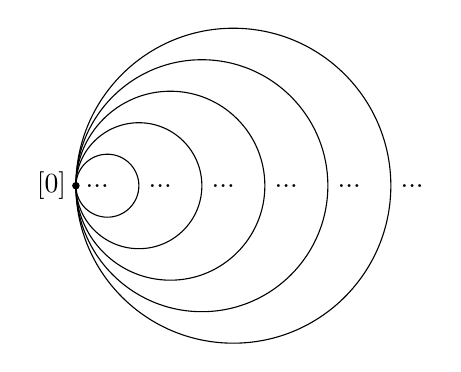
\begin{tikzpicture}[scale=0.4]
        \draw (5,0) circle (5);
        \node[left] at (0,0) {$[0]$};
        \draw[fill] (0,0) circle (0.1);
        \draw (4,0) circle (4);
        \draw (3,0) circle (3);
        \draw (2,0) circle (2);
        \draw (1,0) circle (1);
        \node[right] at (0,0) {...};
        \node[right] at (2,0) {...};
        \node[right] at (4,0) {...};
        \node[right] at (6,0) {...};
        \node[right] at (8,0) {...};
        \node[right] at (10,0) {...};
      \end{tikzpicture}
      \caption{It turns out that every interval $[j, j+1] \subset \mathbb{R}, \; j \in \mathbb{Z}$ will get mapped as a closed loop in $\mathbb{R} / \sim$ beginning and ending with $[0]$, since $j, j+1 \mapsto [0]$. So geometrically, $\mathbb{R} / \sim$ consists of an infinite number of nonintersecting closed loops starting and ending with $[0]$. }
      \label{fig:integer}
    \end{figure}

    This wacky mapping is an example of a quotient mapping that does not preserve topological structure. While it will not be proven here, it is known that $(\mathbb{R}, \T_{\mathbb{R}})$ is 1st and 2nd countable, but $\mathbb{R} / \sim$ under this relation is not even 1st countable. 
  \end{example}

  We now introduce theorems of continuous maps from quotient spaces inducing other continuous maps. 

  \begin{theorem}
    Let $p: (X, \T_X) \rightarrow (Y, \T_Y)$ be a quotient map. Let $(Z, \T_Z)$ be a topological space and let there exist a function $f: Y \rightarrow Z$. $f$ is continuous if and only if $f \circ p$ is continuous. 

    \begin{figure}[H]
      \centering 
      \begin{tikzcd}
        X \arrow{d}{p} \arrow{rd}{f \circ p}\\
        Y \arrow{r}{f} & Z
      \end{tikzcd}
      \label{fig:decomposition_of_continuous}
    \end{figure}

  \end{theorem}
  \begin{proof}
    We prove bidirectionally. 
    \begin{enumerate}
      \item ($\rightarrow$) Assume $f$ is continuous. By definition of the quotient topology, $p$ is continuous $\implies$ $f \circ p$ is continuous. 
      \item ($\leftarrow$) Assume $f \circ p$ is continuous $\iff (f \circ p)^{-1} (\omega) \in \T_X$ for every $\omega \in \T_Z \iff p^{-1} \big( f^{-1}(\omega) \big) \in \T_X$, but $p$ is continuous, so $f^{-1}(\omega)$ is open in $Y$. Therefore, given $\omega \in \T_{Z}$, $f^{-1} (\omega) \in \T_Y \implies f$ is continuous. 
    \end{enumerate}
  \end{proof}

  The previous theorem determines continuity of $f$ and $f \circ p$ given a function mapping $Y \rightarrow Z$. The following analogous theorem determines continuity of an induced map $f$ given a function mapping $X \rightarrow Z$. 

  \begin{theorem}
    Let $p: (X, \T_X )\rightarrow (Y, \T_Y)$ be a quotient map. Let $Z$ be a space and let $g: X \rightarrow Z$ be a map such that $g$ is constant on the elements $x$ of each equivalence class induced by $p$. That is, if $x_1$ and $x_2$ are in the same equivalence class induced by $p$, i.e. 
    \begin{equation}
      p(x_1) = p(x_2)
    \end{equation}
    then $g(x_1) = g(x_2)$. If $g$ is continuous, then $g$ induces a continuous map $f: X \rightarrow Z$ such that $g = f \circ p$. 

    \begin{figure}[H]
      \centering 
      \begin{tikzcd}
        X \arrow{d}{p} \arrow{rd}{g=f \circ p}\\
          Y \arrow{r}{f} & Z
      \end{tikzcd}
      \caption{The theorem states that the diagram commutes. } 
      \label{fig:quotient_continuity}
    \end{figure}

  \end{theorem}

